\chapter{Sterowanie}

\section{Wprowadzenie}
W celu sterowania układem można wykorzystać wiele popularnych algorytmów, od najpopularniejszych typu PID, po bardziej złożone jak np. LQR.

\section{Algorytm sterowania}
Jako algorytm sterowania został wykorzystany regulator proporcjonalnie-całkująco-różniczkujący. Regulator PID został wybrane ze względu na:
\begin{itemize}
    \item mały nakład obliczeń
    \item szybkość działania
    \item bezproblemową implementację w zastosowanym mikrokontrolerze \ref{fig:STM32}.
\end{itemize} 
W pracy został wykorzystany dokładnie regulator PID w wersji IND \textit{(ang.INDedpendent algorithm}, którego transmitancja opisana jest wzorem \ref{eq:pidind}.
\begin{equation}
    G(s)=K_p+K_i\frac{1}{s}+K_ds
    \label{eq:pidind}
\end{equation}
Algorytm regulatora został zaimplementowany w postaci dyskretnej w języku C \ref{fig:pidind}, w celu wykorzystania go w mikrokontrolerze \ref{sec:STM32}.
Cały algorytm składa się z 2 takich regulatorów, które są odpowiedzialne za:
\begin{itemize}
    \item pozycję wózka na osi X,
    \item kąt odchylanie wahadła.
\end{itemize}
Wyjściem sterującym jest różnicą wyjść obu regulatorów. Należy zadbać, aby algorytm odpowiedzialny za odchylenie wahadła działał z większą częstotliwością w porównaniu do drugiego, żeby układ miał szansę działać prawidłowo. W przypadku, gdy nastawy regulatorów zostaną dobrane zbyt agresywne, może to spowodować wzajemne zagłuszanie się, a w konsekwencji nieprawidłowe sterowanie obiektem \cite{odwWah}. 

\begin{figure}
    \centering
    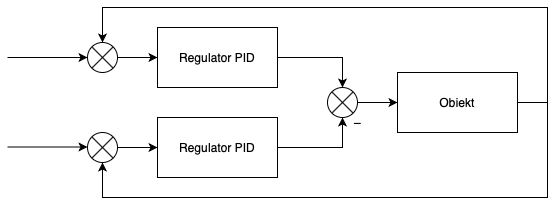
\includegraphics[scale=0.7]{praca_dyplomowa/figures/2xPID.png}
    \caption{Dwa regulatory PID w konfiguracji równoległej}
    \label{fig:sim}
\end{figure}



%\subsection{Dwa regulatory PID szeregowo}
%\subsection{Regulator LQR}



